\subsubsection{UC33-Accettazione prenotazione}
\begin{figure}[h] 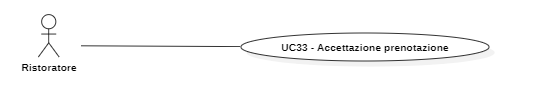
\includegraphics[scale=1]{uc33.png} \end{figure}
\begin{itemize}
\item \textbf{Attore principale:} Ristoratore.
\item \textbf{Precondizioni:}
\begin{itemize}
        \item Il ristoratore è connesso al sistema e sta visualizzando il dettaglio di una singola prenotazione (si veda UC36-Visualizzazione singola prenotazione);
        \item La prenotazione è nello stato "In attesa".
\end{itemize}
\item \textbf{Postcondizioni:} Lo stato della prenotazione diventa "Accettata".
\item \textbf{Scenario principale:}
\begin{enumerate}
    \item Il ristoratore seleziona l'opzione di accettazione della prenotazione;
    \item Il sistema aggiorna lo stato della prenotazione.
\end{enumerate}
\end{itemize}

\pagebreak
\subsubsection{UC34-Rifiuta prenotazione}
\begin{figure}[h] 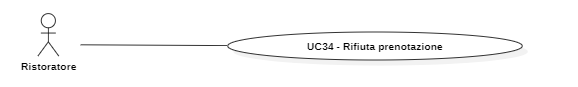
\includegraphics[scale=1]{uc34.png} \end{figure}
\begin{itemize}
\item \textbf{Attore principale:} Ristoratore.
\item \textbf{Precondizioni:}
\begin{itemize}
        \item Il ristoratore è connesso al sistema e sta visualizzando il dettaglio di una singola prenotazione (si veda UC36-Visualizzazione singola prenotazione);
        \item La prenotazione è nello stato "In attesa".
\end{itemize}
\item \textbf{Postcondizioni:} Lo stato della prenotazione diventa "Rifiutata".
\item \textbf{Scenario principale:}
\begin{enumerate}
    \item Il ristoratore seleziona l'opzione di rifiuto della prenotazione;
    \item Il ristoratore inserisce opzionalmente le motivazioni del rifiuto della prenotazione;
    \item Il sistema aggiorna lo stato della prenotazione.
\end{enumerate}
\end{itemize}

\subsubsection{UC35-Visualizzazione lista prenotazioni}
\begin{figure}[h] 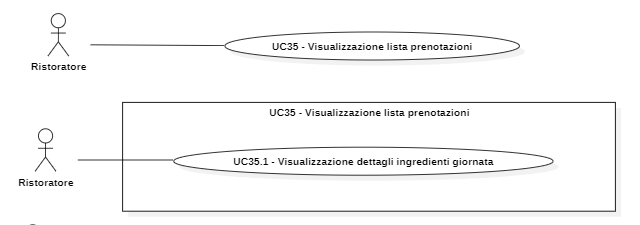
\includegraphics[scale=1]{uc35.png} \end{figure}
\begin{itemize}
\item \textbf{Attore principale:} Ristoratore.
\item \textbf{Precondizioni:} Il ristoratore è connesso al sistema.
\item \textbf{Postcondizioni:} Il ristoratore visualizza la lista delle prenotazioni (in qualsiasi stato esse si trovino) suddivise per giorno.
\item \textbf{Scenario principale:}
\begin{enumerate}
    \item Il sistema mostra le prenotazioni raggruppate per giorno.
    \item Per ogni giorno il ristoratore può consultare:
    \begin{itemize}
        \item La lista delle prenotazioni di quel particolare giorno;
        \item La lista degli ingredienti necessari per tale giorno (si veda UC35.1).
    \end{itemize}
    \item Il sistema mostra la lista delle prenotazioni inerente ad un giorno nei seguenti modi:
    \begin{itemize}
        \item Di default, vengono mostrate come prime le prenotazioni nello stato "Accettata";
        \item Il ristoratore può inoltre applicare un filtro in base allo stato della prenotazione.
    \end{itemize}
\end{enumerate}
\end{itemize}

\subsubsection{UC54-Visualizzazione dettagli ingredienti giornata}
\begin{figure}[h] 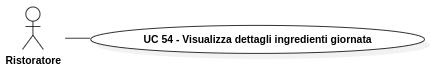
\includegraphics[scale=1]{uc54.png} \end{figure}
\begin{itemize}
\item \textbf{Attore principale:} Ristoratore.
\item \textbf{Precondizioni:} Il ristoratore si trova nella propria dashboard.
\item \textbf{Postcondizioni:} Il ristoratore visualizza la lista degli ingredienti.
\item \textbf{Scenario principale:}
\begin{enumerate}
    \item Il ristoratore seleziona la funzionalità per vedere il dettaglio degli ingredienti necessari per la giornata selezionata da un calendario;
    \item Il sistema mostra la lista degli ingredienti relativi alla giornata, relativamente alle prenotazioni nello stato "Accettata";
    \item Il ristoratore visualizza la lista degli ingredienti.
\end{enumerate}
\end{itemize}

\subsubsection{UC36-Visualizzazione singola prenotazione}
\begin{figure}[h] 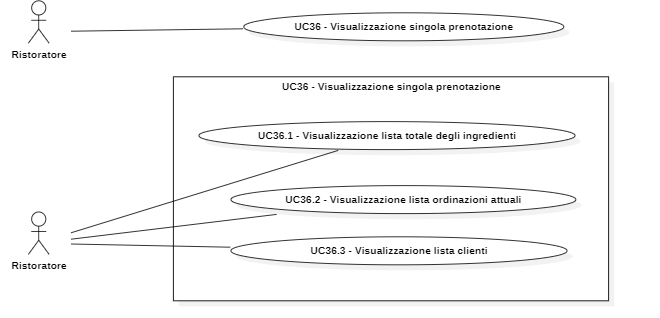
\includegraphics[scale=1]{uc36.png} \end{figure}
\begin{itemize}
    \item \textbf{Attore principale:} Ristoratore.
    \item \textbf{Precondizioni:} Il ristoratore si trova nella sezione "Visualizzazione lista prenotazioni" (si veda UC35);
    \item \textbf{Postcondizioni:} Il ristoratore visualizza le informazioni dettagliate della singola prenotazione.
    \item \textbf{Scenario principale:}
    \begin{enumerate}
        \item Il ristoratore seleziona una prenotazione da visualizzare in dettaglio.
        \item Il sistema mostra i dettagli e le informazioni relative alla prenotazione selezionata dal ristoratore:
        \begin{itemize}
            \item Username del profilo che ha effettuato la prenotazione;
            \item Giorno e orario della prenotazione;
            \item Numero di persone;
            \item Stato della prenotazione;
            \item Lista totale degli ingredienti per la ordinazione (si veda UC36.1);
            \item Lista delle ordinazioni attuali, sia confermate che non (si veda UC36.2);
            \item Lista dei clienti facenti parte della prenotazione (si veda UC36.3).
        \end{itemize}
    \end{enumerate}
\end{itemize}

\textbf{UC36.1-Visualizzazione lista totale degli ingredienti}
\begin{itemize}
    \item \textbf{Attore principale:} Ristoratore.
    \item \textbf{Precondizioni:}
    \begin{itemize}
        \item Il ristoratore si trova nella sezione "Visualizzazione singola prenotazione" (si veda UC36);
        \item Il ristoratore seleziona "Lista ingredienti per questa prenotazione".
    \end{itemize}
    \item \textbf{Postcondizioni:} Il ristoratore visualizza la lista degli ingredienti per la singola prenotazione.
    \item \textbf{Scenario principale:}
    \begin{enumerate}
        \item Il ristoratore visualizza la lista degli ingredienti che servono per completare quella prenotazione, ogni ingrediente ha una sua quantità espressa in grammi.
    \end{enumerate}
\end{itemize}

\textbf{UC36.2-Visualizzazione lista ordinazioni attuali}
\begin{itemize}
    \item \textbf{Attore principale:} Ristoratore.
    \item \textbf{Precondizioni:} Il ristoratore si trova nella sezione "Visualizzazione singola prenotazione" (si veda UC36).
    \item \textbf{Postcondizioni:} Il ristoratore visualizza la lista delle ordinazioni per la singola prenotazione.
    \item \textbf{Scenario principale:}
    \begin{enumerate}
        \item Il ristoratore seleziona l'opzione "Ordinazioni per questa prenotazione";
        \item Il ristoratore visualizza la lista delle ordinazioni che sono state effettuate dai clienti collegati a questa prenotazione nei seguenti modi:
        \begin{itemize}
            \item Di default, vengono mostrate come prime le ordinazioni nello stato "Confermata";
            \item Il ristoratore può inoltre applicare un filtro in base allo stato dell'ordinazione.
        \end{itemize}
    \end{enumerate}
\end{itemize}

\pagebreak

\textbf{UC36.3-Visualizzazione lista Clienti}
\begin{itemize}
    \item \textbf{Attore principale:} Ristoratore.
    \item \textbf{Precondizioni:}
    \begin{itemize}
        \item Il ristoratore si trova nella sezione "Visualizzazione singola prenotazione" (si veda UC36);
        \item Il ristoratore seleziona "Lista clienti".
    \end{itemize}
    \item \textbf{Postcondizioni:} Il ristoratore visualizza la lista dei clienti collegati alla singola prenotazione.
    \item \textbf{Scenario principale:}
    \begin{enumerate}
        \item Il ristoratore visualizza la lista dei clienti collegati a questa prenotazione nei seguenti modi:
        \begin{itemize}
            \item Di default, vengono mostrati per primi i clienti le cui ordinazioni sono nello stato "Confermata";
            \item Il ristoratore può inoltre applicare un filtro in base allo stato dell'ordinazione del cliente.
        \end{itemize}
    \end{enumerate}
\end{itemize}

\subsubsection{UC37-Modifica menù}
\begin{figure}[h] 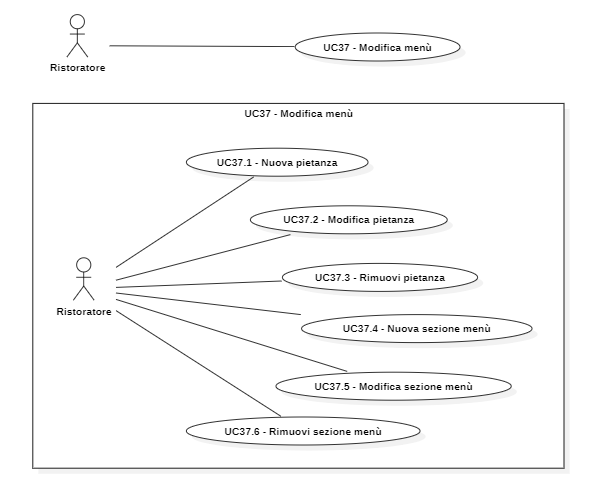
\includegraphics[scale=1]{uc37.png} \end{figure}
\begin{itemize}
    \item \textbf{Attore principale:} Ristoratore.
    \item \textbf{Precondizioni:} Il ristoratore ha effettuato l'accesso al sistema.
    \item \textbf{Postcondizioni:} Le modifiche apportate al menù sono salvate.
    \item \textbf{Scenario principale:}
    \begin{enumerate}
        \item Il ristoratore visualizza le pietanze contenute nel menù del ristorante;
        \item Il ristoratore può eseguire le seguenti operazioni di modifica:
        \begin{itemize}
           \item Aggiungere una nuova pietanza al menù (si veda UC37.1);
           \item Modificare una pietanza preesistente (si veda UC37.2);
           \item Rimuovere una pietanza dal menù (si veda UC37.3);
           \item Aggiungere una nuova sezione al menù (si veda UC37.4);
           \item Modificare una sezione del menù (si veda UC37.5);
           \item Rimuovere una sezione dal menù (si veda UC37.6);
        \end{itemize}
        \item Il ristoratore dopo aver apportato modifiche al menù le conferma;
        \item Il sistema aggiorna le informazioni sul menù del ristorante;
    \end{enumerate}
\end{itemize}

\textbf{UC37.1-Nuova pietanza}
\begin{itemize}
    \item \textbf{Attore principale:} Ristoratore.
    \item \textbf{Precondizioni:} Il ristoratore si trova nella sezione di modifica del menù (si veda UC37).
    \item \textbf{Postcondizioni:} Il ristoratore ha inserito una nuova pietanza al menù.
    \item \textbf{Scenario principale:}
    \begin{enumerate}
        \item Il ristoratore seleziona l'opzione di creazione di una nuova pietanza;
        \item Il ristoratore inserisce le informazioni relative alla pietanza:
        \begin{itemize}
            \item Il nome della pietanza;
            \item Seleziona gli ingredienti che compongono la pietanza dalla lista degli ingredienti, con la loro quantità espressa in grammi (si veda UC38 per la creazione di tale lista);
            \item Seleziona la sezione del menù a cui questo piatto appartiene.
        \end{itemize}
        \item Il ristoratore conferma l'aggiunta di una nuova pietanza al menù;
        \item Il sistema aggiorna il menù con la nuova pietanza;
        \item Il ristoratore viene reindirizzato alla schermata di modifica menù (si veda UC37).
    \end{enumerate}
\end{itemize}

\textbf{UC37.2-Modifica pietanza}
\begin{itemize}
    \item \textbf{Attore principale:} Ristoratore.
    \item \textbf{Precondizioni:} Il ristoratore si trova nella sezione di modifica del menù (si veda UC37).
    \item \textbf{Postcondizioni:} Il ristoratore ha modificato una pietanza al menù.
    \item \textbf{Scenario principale:}
    \begin{enumerate}
        \item Il ristoratore seleziona l'opzione di modifica di una pietanza;
        \item Il ristoratore modifica le informazioni relative alla pietanza:
        \begin{itemize}
            \item Il nome della pietanza;
            \item Seleziona gli ingredienti che compongono la pietanza dalla lista degli ingredienti, con la loro quantità espressa in grammi (si veda UC38 per la creazione di tale lista);
            \item Seleziona la sezione del menù a cui questo piatto appartiene.
        \end{itemize}
        \item Il ristoratore conferma le modifiche della pietanza;
        \item Il sistema aggiorna il menù con le modifiche apportate alla pietanza;
        \item Il ristoratore viene reindirizzato alla schermata di modifica menù (si veda UC37).
    \end{enumerate}
\end{itemize}

\textbf{UC37.3-Rimuovi pietanza}
\begin{itemize}
    \item \textbf{Attore principale:} Ristoratore.
    \item \textbf{Precondizioni:} Il ristoratore si trova nella sezione di modifica del menù (si veda UC37).
    \item \textbf{Postcondizioni:} La pietanza non è più presente nel menù.
    \item \textbf{Scenario principale:}
    \begin{enumerate}
        \item Il ristoratore seleziona l'opzione di eliminazione di una pietanza;
        \item Il sistema aggiorna il menù con l'eliminazione della pietanza.
        \item Il ristoratore viene reindirizzato alla schermata di modifica menù (si veda UC37).
    \end{enumerate}
\end{itemize}


\textbf{UC37.4-Nuova sezione menù}
\begin{itemize}
    \item \textbf{Attore principale:} Ristoratore.
    \item \textbf{Precondizioni:} Il ristoratore si trova nella sezione di modifica del menù (si veda UC37).
    \item \textbf{Postcondizioni:} Il ristoratore ha inserito una nuova sezione al menù.
    \item \textbf{Scenario principale:}
    \begin{enumerate}
        \item Il ristoratore seleziona l'opzione di creazione di una sezione;
        \item Il ristoratore inserisce il nome della nuova sezione;
        \item Il ristoratore conferma l'aggiunta di una nuova sezione al menù;
        \item Il sistema aggiorna il menù con la nuova seziona inserita.
    \end{enumerate}
\end{itemize}

\textbf{UC37.5-Modifica sezione menù}
\begin{itemize}
    \item \textbf{Attore principale:} Ristoratore.
    \item \textbf{Precondizioni:} Il ristoratore si trova nella sezione di modifica del menù (si veda UC37).
    \item \textbf{Postcondizioni:} Il ristoratore ha modificato una sezione al menù.
    \item \textbf{Scenario principale:}
    \begin{enumerate}
        \item Il ristoratore seleziona l'opzione di modifica di una sezione;
        \item Il ristoratore modifica il nome della sezione;
        \item Il ristoratore conferma le modifiche apportate alla sezione;
        \item Il sistema aggiorna il menù con la sezione modificata dal ristoratore.
    \end{enumerate}
\end{itemize}


\textbf{UC37.6-Rimuovi sezione menù}
\begin{itemize}
    \item \textbf{Attore principale:} Ristoratore.
    \item \textbf{Precondizioni:} Il ristoratore si trova nella sezione di modifica del menù (si veda UC37).
    \item \textbf{Postcondizioni:} La sezione non è più presente nel menù.
    \item \textbf{Scenario principale:}
    \begin{enumerate}
        \item Il ristoratore seleziona l'opzione di eliminazione di una sezione;
        \item Il sistema aggiorna il menù con l'eliminazione della sezione.
    \end{enumerate}
\end{itemize}

\subsubsection{UC38-Modifica lista degli ingredienti}
\begin{figure}[h] 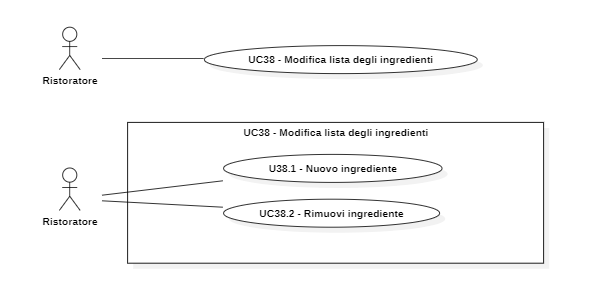
\includegraphics[scale=1]{uc38.png} \end{figure}
\begin{itemize}
    \item \textbf{Attore principale:} Ristoratore.
    \item \textbf{Precondizioni:} Il ristoratore ha effettuato l'accesso al sistema.
    \item \textbf{Postcondizioni:} Le modifiche apportate sono state salvate.
    \item \textbf{Scenario principale:}
    \begin{enumerate}
        \item Il ristoratore visualizza la lista degli ingredienti del ristorante;
        \item Il ristoratore può eseguire le seguenti operazioni:
        \begin{itemize}
           \item Aggiungere un nuovo ingrediente alla lista (si veda UC38.1);
           \item Rimuovere un ingrediente presente nella lista (si veda UC38.2).
        \end{itemize}
    \item Il ristoratore conferma le modifiche apportate alla lista degli ingredienti;
    \item Il sistema aggiorna la lista degli ingredienti;
    \item Il ristoratore viene reindirizzato alla dashboard.
    \end{enumerate}
\end{itemize}

\pagebreak
\textbf{UC38.1-Nuovo ingrediente}
\begin{itemize}
    \item \textbf{Attore principale:} Ristoratore.
    \item \textbf{Precondizioni:} Il ristoratore si trova nella sezione di modifica della lista ingredienti (si veda UC38).
    \item \textbf{Postcondizioni:} Viene inserito un nuovo ingrediente nella lista degli ingredienti.
    \item \textbf{Scenario principale:}
    \begin{enumerate}
        \item Il ristoratore seleziona l'opzione di creazione di un nuovo ingrediente;
        \item Il ristoratore compila il seguente form contenente le informazioni relative alla pietanza:
        \begin{itemize}
            \item Il nome dell'ingrediente;
            \item Opzionalmente seleziona gli allergeni contenuti all'interno di quell'ingrediente da una lista fornita dal sistema.
        \end{itemize}
        \item Il ristoratore conferma la creazione di un nuovo ingrediente;
        \item Il sistema aggiorna la lista degli ingredienti con il nuovo ingrediente;
        \item Il ristoratore viene reindirizzato alla schermata di modifica della lista ingredienti (si veda UC38).
    \end{enumerate}
\end{itemize}


\textbf{UC38.2-Rimuovi ingrediente}
\begin{itemize}
    \item \textbf{Attore principale:} Ristoratore.
    \item \textbf{Precondizioni:} Il ristoratore si trova nella sezione di gestione della lista ingredienti (si veda UC38).
    \item \textbf{Postcondizioni:} L'ingrediente viene rimosso dalla lista degli ingredienti.
    \item \textbf{Scenario principale:}
    \begin{enumerate}
        \item Il ristoratore seleziona l'opzione di eliminazione un ingrediente;
        \item Il sistema aggiorna la lista con l'eliminazione dell'ingrediente;
        \item Il ristoratore viene reindirizzato alla schermata di modifica della lista ingredienti (si veda UC38).
    \end{enumerate}
\end{itemize}
\pagebreak
\subsubsection{UC39-Visualizzazione recensioni ristorante} % analizzare più in dettaglio (grazie al *****)
\begin{figure}[h] 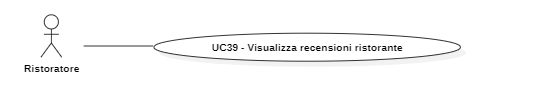
\includegraphics[scale=1]{uc39.png} \end{figure}
\begin{itemize}
\item \textbf{Attore principale:} Ristoratore.
\item \textbf{Precondizioni:} Il ristoratore si trova nella dashboard.
\item \textbf{Postcondizioni:} Il ristoratore visualizza le ultime 5 recensioni fatte in ordine temporale decrescente dai clienti.
\item \textbf{Scenario principale:}
\begin{enumerate}
    \item Il ristoratore seleziona la funzionalità di visualizzazione delle recensioni fatte dai clienti sulla loro esperienza presso il ristorante;
    \item Il sistema presenta la lista delle recensioni fatte in ordine temporale decrescente;
    \item Il ristoratore visualizza le seguenti informazioni per ogni recensione:
    \begin{itemize}
        \item Il nome del profilo che l'ha rilasciata;
        \item La timestamp di rilascio;
        \item Un voto da 1 a 5 sul menù;
        \item Un voto da 1 a 5 sul servizio;
        \item Un voto da 1 a 5 sul prezzo;
        \item Un eventuale commento testuale.
    \end{itemize}
\end{enumerate}
\end{itemize}

\subsubsection{UC40-Gestione pagamento conto}
\begin{figure}[h] 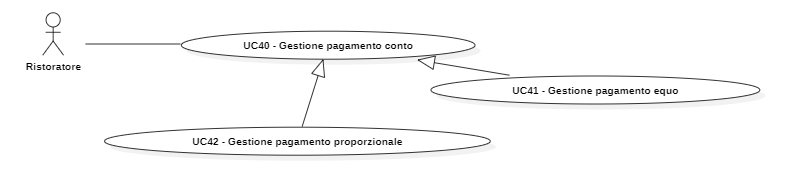
\includegraphics[scale=.7]{uc40.png} \end{figure}
\begin{itemize}
    \item \textbf{Attore principale:} Ristoratore.
    \item \textbf{Precondizioni:}
    \begin{itemize}
        \item Il ristoratore è connesso al sistema e si trova nella sezione di visualizzazione di una singola prenotazione (si veda UC36);
        \item Un cliente ha selezionato la modalità di divisione del conto (si veda UC27).
    \end{itemize}
    \item \textbf{Postcondizioni:} Rispettando la modalità di divisione del conto, una parte o il totale del conto della prenotazione è segnato come pagato.
    \item \textbf{Scenario principale:}
    \begin{enumerate}
        \item Il sistema mostra gli ordini o le persone nello stato "Pagato" e "Non pagato", elencando per prime quelle nello stato "Non pagato";
        \item Il ristoratore può selezionare un ordine o una persona e segnarla come pagata;
        \item Il sistema aggiorna lo stato dell'ordine o della persona a "Pagato";
        \item Quando tutte le ordinazioni o persone hanno pagato allora la prenotazione va nello stato "Pagata".
    \end{enumerate}
    \item \textbf{Specializzazioni:}
        \begin{itemize}
            \item UC41-Pagamento equo;
            \item UC42-Pagamento proporzionale.
        \end{itemize}
\end{itemize}

\subsubsection{UC41-Gestione pagamento equo}
\begin{itemize}
    \item \textbf{Descrizione:} Pagamento equo del totale di tutti gli ordini, ovvero "alla romana".
    \item \textbf{Attore principale:} Ristoratore.
    \item \textbf{Precondizioni:}
    \begin{itemize}
        \item Il ristoratore è connesso al sistema e si trova nella sezione di visualizzazione di una singola prenotazione (si veda UC36);
        \item Un cliente ha selezionato la modalità di divisione del conto equa (si veda UC27).
    \end{itemize}
    \item \textbf{Postcondizioni:} Il o i profili selezionati sono segnati come pagati.
    \item \textbf{Scenario principale:}
    \begin{enumerate}
        \item Il sistema mostra le persone nello stato "Pagato" e "Non pagato", elencando per prime quelle nello stato "Non pagato";
        \item Il ristoratore può selezionare una persona o più persone e segnarle come pagate;
        \item Il sistema aggiorna lo stato delle persone a "Pagato";
        \item Quando tutte le persone hanno pagato allora la prenotazione va nello stato "Pagata".
    \end{enumerate}
\end{itemize}

\subsubsection{UC42-Gestione pagamento proporzionale}
\begin{itemize}
    \item \textbf{Descrizione:} Pagamento proporzionale delle ordinazioni, ovvero i clienti selezionano gli ordini che vogliono pagare (anche di altri clienti).
    \item \textbf{Attore principale:} Ristoratore.
    \begin{itemize}
        \item Il ristoratore è connesso al sistema e si trova nella sezione di visualizzazione di una singola prenotazione (si veda UC36);
        \item Un cliente ha selezionato la modalità di divisione del conto proporzionale (si veda UC27).
    \end{itemize}
    \item \textbf{Postcondizioni:} Una o più ordinazioni selezionate sono segnate come pagate.
    \item \textbf{Scenario principale:}
    \begin{enumerate}
        \item Il sistema mostra le ordinazioni nello stato "Pagato" e "Non pagato", elencando per prime quelle nello stato "Non pagato";
        \item Il ristoratore può selezionare una o più ordinazioni e segnarle come pagate;
        \item Il sistema aggiorna lo stato delle ordinazioni a "Pagato";
        \item Quando tutte le ordinazioni sono segnate come pagate allora la prenotazione va nello stato "Pagato".
    \end{enumerate}
\end{itemize}

\subsubsection{UC43-Visualizzazione notifica cliente ha confermato l'ordinazione}
\begin{figure}[h] 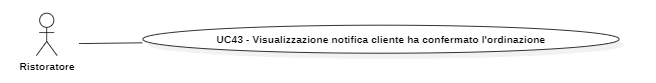
\includegraphics[scale=1]{uc43.png} \end{figure}
\begin{itemize}
\item \textbf{Attore principale:} Ristoratore.
\item \textbf{Precondizioni:} Il cliente ha confermato l'ordinazione (si veda UC23.3).
\item \textbf{Postcondizioni:} Il ristoratore visualizza una notifica relativa alla conferma dell'ordinazione.
\item \textbf{Scenario principale:}
\begin{enumerate}
    \item Il sistema vede che è stata confermata un'ordinazione dal cliente;
    \item Il sistema invia al ristoratore una notifica relativa alla conferma dell'ordinazione;
    \item Il ristoratore visualizza la notifica relativa all'ordinazione.
\end{enumerate}
\end{itemize}

\subsubsection{UC44-Visualizzazione notifica cliente ha annullato la prenotazione}
\begin{figure}[h] 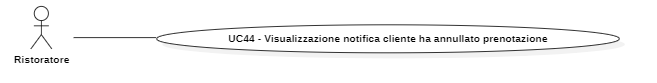
\includegraphics[scale=1]{uc44.png} \end{figure}
\begin{itemize}
\item \textbf{Attore principale:} Ristoratore.
\item \textbf{Precondizioni:} Il cliente ha annullato la prenotazione (si veda UC21).
\item \textbf{Postcondizioni:} Il ristoratore visualizza una notifica relativa all'annullamento della prenotazione.
\item \textbf{Scenario principale:}
\begin{enumerate}
    \item Il sistema vede che è stata annullata una prenotazione dal cliente;
    \item Il sistema invia al ristoratore una notifica relativa all'annullamento della prenotazione;
    \item Il ristoratore visualizza la notifica relativa all'annullamento della prenotazione.
\end{enumerate}
\end{itemize}

\pagebreak
\subsubsection{UC45-Visualizzazione notifica nuova prenotazione in arrivo}
\begin{figure}[h] 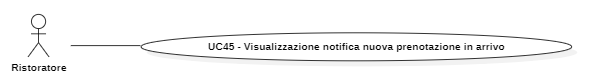
\includegraphics[scale=1]{uc45.png} \end{figure}
\begin{itemize}
\item \textbf{Attore principale:} Ristoratore.
\item \textbf{Precondizioni:} Il cliente ha effettuato una prenotazione (si veda UC19).
\item \textbf{Postcondizioni:} Il ristoratore visualizza una notifica relativa alla prenotazione di un tavolo.
\item \textbf{Scenario principale:}
\begin{enumerate}
    \item Il sistema vede che è stata effettuata una prenotazione dal cliente;
    \item Il sistema invia al ristoratore una notifica relativa ad una nuova prenotazione;
    \item Il ristoratore visualizza la notifica relativa alla nuova prenotazione.
\end{enumerate}
\end{itemize}

\subsubsection{UC46-Visualizzazione notifica nuova recensione}
\begin{figure}[h] 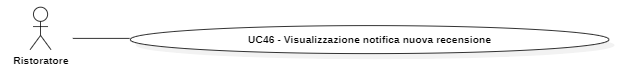
\includegraphics[scale=1]{uc46.png} \end{figure}
\begin{itemize}
\item \textbf{Attore principale:} Ristoratore.
\item \textbf{Precondizioni:} Il cliente ha lasciato una recensione (si veda UC29).
\item \textbf{Postcondizioni:} Il ristoratore visualizza una notifica relativa alla recensione.
\item \textbf{Scenario principale:}
\begin{enumerate}
    \item Il sistema vede che è stata lasciata una recensione dal cliente;
    \item Il sistema invia al ristoratore una notifica relativa alla nuova recensione;
    \item Il ristoratore visualizza la notifica relativa alla nuova recensione.
\end{enumerate}
\end{itemize}

\pagebreak
\subsubsection{UC47-Visualizzazione notifica cliente ha pagato in app}
\begin{figure}[h] 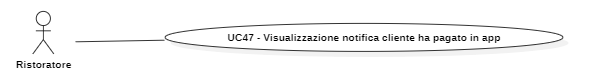
\includegraphics[scale=1]{uc47.png} \end{figure}
\begin{itemize}
\item \textbf{Attore principale:} Ristoratore.
\item \textbf{Precondizioni:} Il cliente ha effettuato un pagamento in app (si veda UC28).
\item \textbf{Postcondizioni:} Il ristoratore visualizza una notifica relativa al pagamento in app.
\item \textbf{Scenario principale:}
\begin{enumerate}
    \item Il sistema vede che è stata pagata un'ordinazione dal cliente;
    \item Il sistema invia al ristoratore una notifica relativa ad un pagamento;
    \item Il ristoratore visualizza la notifica relativa al pagamento.
\end{enumerate}
\end{itemize}

\subsubsection{UC48-Visualizzazione notifica ricezione messaggio in chat}
\begin{figure}[h] 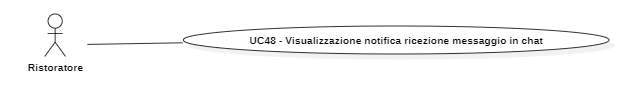
\includegraphics[scale=1]{uc48.png} \end{figure}
\begin{itemize}
\item \textbf{Attore principale:} Ristoratore.
\item \textbf{Precondizioni:}
\begin{itemize}
    \item Il cliente ha avviato la chat con il ristoratore (si veda UC49);
    \item Il cliente ha inviato un messaggio al ristoratore (si veda UC50.1).
\end{itemize}
\item \textbf{Postcondizioni:} Il ristoratore visualizza una notifica relativa alla ricezione di un messaggio in chat.
\item \textbf{Scenario principale:}
\begin{enumerate}
    \item Il sistema vede che è stato inviato un messaggio dal cliente;
    \item Il sistema invia al ristoratore una notifica relativa al messaggio;
    \item Il ristoratore visualizza la notifica relativa al messaggio.
\end{enumerate}
\end{itemize}


